% This must be in the first 5 lines to tell arXiv to use pdfLaTeX, which is strongly recommended.
% In particular, the hyperref package requires pdfLaTeX in order to break URLs across lines.

\documentclass[11pt]{article}

% Remove the "review" option to generate the final version.
\usepackage[review]{acl}

% Standard package includes
\usepackage{times, graphicx}
\usepackage{latexsym}

% For proper rendering and hyphenation of words containing Latin characters (including in bib files)
\usepackage[T1]{fontenc}
% For Vietnamese characters
% \usepackage[T5]{fontenc}
% See https://www.latex-project.org/help/documentation/encguide.pdf for other character sets

% This assumes your files are encoded as UTF8
\usepackage[utf8]{inputenc}

% This is not strictly necessary, and may be commented out,
% but it will improve the layout of the manuscript,
% and will typically save some space.
\usepackage{microtype}

% If the title and author information does not fit in the area allocated, uncomment the following
%
%\setlength\titlebox{<dim>}
%
% and set <dim> to something 5cm or larger.

\title{COMP0084 Coursework 1}

% Author information can be set in various styles:
% For several authors from the same institution:
% \author{Author 1 \and ... \and Author n \\
%         Address line \\ ... \\ Address line}
% if the names do not fit well on one line use
%         Author 1 \\ {\bf Author 2} \\ ... \\ {\bf Author n} \\
% For authors from different institutions:
% \author{Author 1 \\ Address line \\  ... \\ Address line
%         \And  ... \And
%         Author n \\ Address line \\ ... \\ Address line}
% To start a seperate ``row'' of authors use \AND, as in
% \author{Author 1 \\ Address line \\  ... \\ Address line
%         \AND
%         Author 2 \\ Address line \\ ... \\ Address line \And
%         Author 3 \\ Address line \\ ... \\ Address line}

\author{First Author \\
  Affiliation / Address line 1 \\
  Affiliation / Address line 2 \\
  Affiliation / Address line 3 \\
  \texttt{email@domain} \\\And
  Second Author \\
  Affiliation / Address line 1 \\
  Affiliation / Address line 2 \\
  Affiliation / Address line 3 \\
  \texttt{email@domain} \\}

\begin{document}
\maketitle
\begin{abstract}
None
\end{abstract}


\section{Task 1: Evaluating Retrieval Quality}

\subsection{Text Processing}
We preprocess passages/queries in two files: \textsl{validation\_data.tsv} and \textsl{train\_data.tsv} by following steps:
\begin{enumerate}
    \item remove url.
    \item lower characters.
    \item remove non alpha characters.
    \item tokenization by Python package NLTK.
\end{enumerate}
\subsection{BM25 Model}
BM25 Model with parameters implemented in the Coursework 1 is used to retrieval the top passages for each query. Here we retrieval top 3, 10 and 100 passages from 1000 passages. The complete result of BM25 model is in \textsl{bm25\_raw\_top1000.tsv}, while we retrieval top 3 passages for each query in \textsl{bm25\_ordered\_top3.tsv}, top 10 passages in \textsl{bm25\_ordered\_top10.tsv} and top 100 passages in \textsl{bm25\_ordered\_top100.tsv}.
\subsection{Metrics}

\subsubsection{Average Precision (AP)}
AP is the average precision of relevant passages for a query.
\begin{equation}
    A P=\frac{\sum_{k=1}^n P(k) \times r e l(k)}{N}
\end{equation}
N: number of relevant passages for the query.\\
k: rank of the passage.
\subsubsection{Mean AP}
Mean AP is the average of AP over all queries.
\begin{equation}
    m A P=\frac{\sum_{q=1}^{N_q} A P_q}{N_q}
\end{equation}
$q$: the $q_{th}$ query
\subsubsection{Discounter Cumulative Gain (DCG)}
DCG is the total gain accumulated at a particular rank p.
\begin{equation}
    D C G_q=\sum_{i=1}^q \frac{2^{r e l_i}-1}{\log _2(i+1)}
\end{equation}
$p$: particular ranking length\\
$i$: the ith passage\\
$rel_i$: relevance score
\subsubsection{Normalized DCG (NDCG)}
Normalizes DCG against the best possible DCG result (the  perfect ranking) for a query.
\begin{equation}
    N D C G_q=\frac{D C G_q}{o p t D C G_q}
\end{equation}
\subsubsection{Mean NDCG}
Mean NDCG is the average of NDCG over all queries.
\begin{equation}
    m NDCG=\frac{\sum_{q=1}^{N_q} N D C G_q}{N_q}
\end{equation}
$N_q$: number of queries\\
The results of the metrics of BM25 model are in Table \ref{tab:bm25}.

\begin{table}[ht]
    \centering
    \caption{Metrics of BM25 model}
    \label{tab:bm25}
    \begin{tabular}{|c|c|c|c|}
        \hline
        BM25 & Cutoff & mAP & mNDCG \\
        \hline
        Top 3 & 3 & 0.1830 & 0.2007 \\
        \hline
        Top 10 & 10 & 0.2250 & 0.2870 \\
        \hline
        Top 100 & 100 & 0.2367 & 0.3548 \\
        \hline
    \end{tabular}
\end{table}
\section{Task 2: Logistic Regression}
\subsection{Subsample}
The train data set is unbalanced (1\% positive, 99\% negative). To balance the data set and reduce the training time, we subsample the negative data set to 20 passages per query and keep all positive passages. For these queries with less than 20 negative passages, we keep all negative passages. The subsampled data set has 95874 passages for 1000 queries.
\subsection{Word Embedding}
We choose Word2Vec to generate word embedding for each term in the vocabulary. The word embedding is a 100-dimensional vector. We use the pre-trained word embedding and set the window size to 5. The word embedding is trained on train and validation data set separately.
\subsection{Logistic Regression}
Logistic function:
\begin{equation}
\sigma_{\mathbf{w}}\left(\mathbf{x}_i\right)=\left(1+e^{-\mathbf{w}^{\top} \mathbf{x}_i}\right)^{-1}
\end{equation}
with weight $w$. The loss function is cross-entropy loss function $\mathcal{J}(\mathbf{w})$:
\begin{equation}
-\frac{1}{n} \sum_{i=1}^n\left[y_i \ln \left(\sigma_w\left(x_i\right)\right)+ \\
\left(1-y_i\right) \ln \left(1-\sigma_w\left(x_i\right)\right)\right]
\end{equation}
The gradient of the loss function is:
\begin{equation}
\frac{\partial \mathcal{J}(\mathbf{w})}{\partial \mathbf{w}_j} = -\frac{1}{n} \sum_{i=1}^n\left[x_{i, j}(y_i-\sigma_w\left(x_i\right)\right]
\end{equation}
We use batch stochastic gradient descent to train the model and stop our training when the validation loss does not decrease for 3 epochs. The word embedding of a query-passage pair given by two vectors with 100 dimensions. We concatenate the two vectors and add a bias term to the model and get a 201-dimensional vector.
\\\\
We initialize the weight vector with 0, set the batch size to 5000, the tolerance to 1e-8, and the maximum number of epochs to 100. To assess the effect of learning rate on our training, we vary the learning rate from 0.01 to 0.0001 and plot the training loss curve in Fig \ref{fig:lr_100}. A larger learning rate results in faster convergence and smaller train loss in the initial epoch. However, all the learning rates converge to the same loss value (0.2) after 100 epochs, except for 0.0001, which still shows no sign of convergence. To confirm convergence, we train the model with 0.0001 for 1000 epochs and present the results in Fig \ref{fig:lr_1000}. The loss converges to 0.2 within 1000 epochs.
\\\\
We decide to use a learning rate of 0.005, batch size of 5000, and epoch number of 100 for the remaining training. Table \ref{tab:lr_metrics} displays the metrics of the model on the validation set.
\\\\
We set the cutoff to 100 and apply the model to predict the relevance scores of passages for each query in the file \textsl{candidate\_passages\_top100.tsv}. We save the top 100 highest-scoring passages for each query in a file called \textsl{LR.csv}.

\begin{figure}
    \centering
    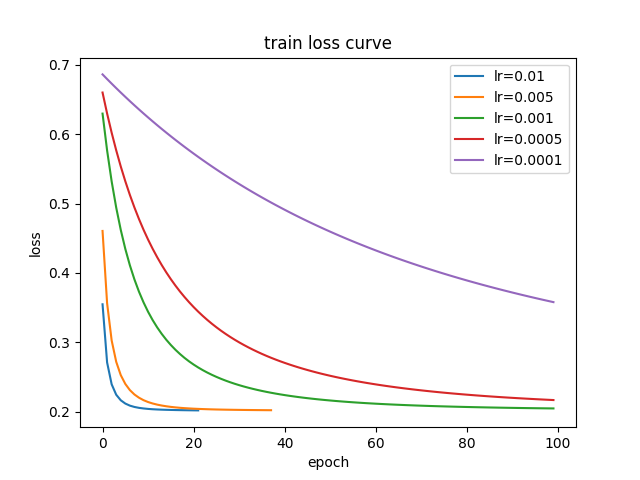
\includegraphics[width=0.5\textwidth]{aseets/epochto100.png}
    \caption{Training loss curve}
    \label{fig:lr_100}
\end{figure}
\begin{figure}
    \centering
    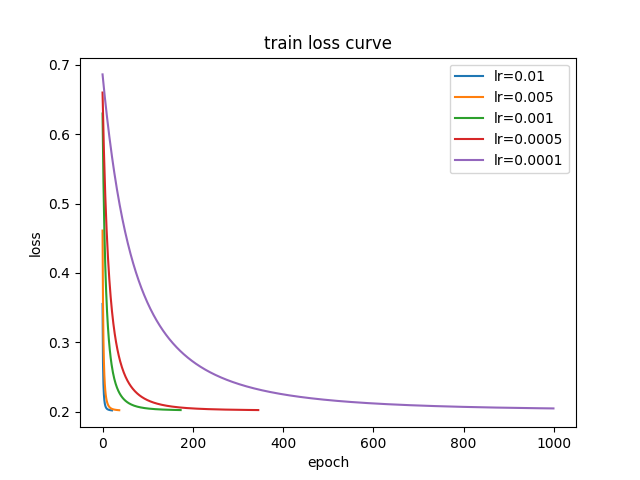
\includegraphics[width=0.5\textwidth]{aseets/epochto1000.png}
    \caption{Training loss curve}
    \label{fig:lr_1000}
\end{figure}
\begin{table}[ht]
    \centering
    \caption{Metrics of LR model}
    \label{tab:lr_metrics}
    \begin{tabular}{|c|c|c|c|}
        \hline
        LR & Cutoff & mAP & mNDCG \\
        \hline
        Top 100 & 100 & 0.0090 & 0.1254 \\
        \hline
    \end{tabular}
\end{table}
\section{Task 3: LambdaMART Model}
\subsection{Model}
Queries and passages is embeded in the same way as in Task 2. However, we replace the bias term with the relevance of the pair passage-query. The input vector is the same as in Task 2 (embedding vector with 201 dimensions) and the label is the relevance of pair passage-query, 0 or 1. The model is trained using the LambdaMART algorithm using some hyper-parameters.

\subsection{Hyper-parameter Tuning}
The objective of the model is \textsl{rank:ndcg} which use LambdaMART to perform list-wise ranking where Normalized Discounted Cumulative Gain (NDCG) is maximized. We use \textsl{gbtree} as the booster. The hyper-parameters are tuned using the validation set. The hyper-parameters are learning rate, number of gradient boosted trees and maximum tree depth for base learners. The metrics mAP and mNDCG of top 100 passages are used to evaluate the model. The grid search method is used to find the best hyper-parameters among the following values: learning rate = 0.0005, 0.001, 0.005, 0.01, 0.05; number of gradient boosted trees = 100, 200, 300; maximum tree depth = 5, 6, 7. The results are shown in Table \ref{tab:hyperparameter_tuning}. The hyper-parameters resulting in the highest mNDCG are learning rate = 0.005, number of gradient boosted trees = 300 and maximum tree depth = 5. The mAP and mNDCG of top 100 passages are 0.0149 and 0.0388 respectively. According to the metrics on the validation data, LambdaMART model with the hyper-parameters above is not as good as previous models.
\begin{center}
    \begin{tabular}{cccccc}
    \hline
    \textbf{No.} & \textbf{eta} & \textbf{depths} & \textbf{n\_ests} & \textbf{mAP} & \textbf{mNDCG} \\
    \hline
    0  & 0.0005 & 5 & 100 & 0.0113 & 0.0301 \\
    1  & 0.0005 & 5 & 200 & 0.0106 & 0.0301 \\
    2  & 0.0005 & 5 & 300 & 0.0095 & 0.0295 \\
    3  & 0.0005 & 6 & 100 & 0.0096 & 0.0292 \\
    4  & 0.0005 & 6 & 200 & 0.0080 & 0.0289 \\
    5  & 0.0005 & 6 & 300 & 0.0093 & 0.0308 \\
    6  & 0.0005 & 7 & 100 & 0.0111 & 0.0289 \\
    7  & 0.0005 & 7 & 200 & 0.0108 & 0.0277 \\
    8  & 0.0005 & 7 & 300 & 0.0102 & 0.0282 \\
    9  & 0.0010 & 5 & 100 & 0.0104 & 0.0313 \\
    10 & 0.0010 & 5 & 200 & 0.0114 & 0.0316 \\
    11 & 0.0010 & 5 & 300 & 0.0130 & 0.0332 \\
    12 & 0.0010 & 6 & 100 & 0.0095 & 0.0315 \\
    13 & 0.0010 & 6 & 200 & 0.0112 & 0.0307 \\
    14 & 0.0010 & 6 & 300 & 0.0085 & 0.0293 \\
    15 & 0.0010 & 7 & 100 & 0.0128 & 0.0315 \\
    16 & 0.0010 & 7 & 200 & 0.0116 & 0.0306 \\
    17 & 0.0010 & 7 & 300 & 0.0105 & 0.0316 \\
    18 & 0.0050 & 5 & 100 & 0.0103 & 0.0340 \\
    19 & 0.0050 & 5 & 200 & 0.0122 & 0.0337 \\
    \hline
    20 & 0.0050 & 5 & 300 & 0.0149 & 0.0388 \\
    \hline
    21 & 0.0050 & 6 & 100 & 0.0127 & 0.0327 \\
    22 & 0.0050 & 6 & 200 & 0.0111 & 0.0291 \\
    23 & 0.0050 & 6 & 300 & 0.0115 & 0.0302 \\
    24 & 0.0050 & 7 & 100 & 0.0086 & 0.0333 \\
    25 & 0.0050 & 7 & 200 & 0.0100 & 0.0340 \\
    26 & 0.0050 & 7 & 300 & 0.0111 & 0.0360 \\
    27 & 0.0100 & 5 & 100 & 0.0096 & 0.0296 \\
    28 & 0.0100 & 5 & 200 & 0.0148 & 0.0367 \\
    29 & 0.0100 & 5 & 300 & 0.0139 & 0.0369 \\
    30 & 0.0100 & 6 & 100 & 0.0074 & 0.0265 \\
    31 & 0.0100 & 6 & 200 & 0.0095 & 0.0287 \\
    32 & 0.0100 & 6 & 300 & 0.0099 & 0.0305 \\
    33 & 0.0100 & 7 & 100 & 0.0110 & 0.0336 \\
    34 & 0.0100 & 7 & 200 & 0.0118 & 0.0321 \\
    35 & 0.0100 & 7 & 300 & 0.0121 & 0.0331 \\
    36 & 0.0500 & 5 & 100 & 0.0096 & 0.0320 \\
    37 & 0.0500 & 5 & 200 & 0.0090 & 0.0324 \\
    38 & 0.0500 & 5 & 300 & 0.0101 & 0.0339 \\
    39 & 0.0500 & 6 & 100 & 0.0119 & 0.0349 \\
    40 & 0.0500 & 6 & 200 & 0.0126 & 0.0358 \\
    41 & 0.0500 & 6 & 300 & 0.0125 & 0.0359 \\
    42 & 0.0500 & 7 & 100 & 0.0134 & 0.0352 \\
    43 & 0.0500 & 7 & 200 & 0.0153 & 0.0393 \\
    44 & 0.0500 & 7 & 300 & 0.0119 & 0.0381 \\
    \hline
    \label{tab:hyperparameter_tuning}
    \end{tabular}
\end{center}


\end{document}
